\begin{proofbox}
\textbf{\textcolor{CProof}{思路提示}} 从平方非负出发，保留原文四步主线：展开、根式代换、两条变形分支。
\begin{description}[style=nextline,leftmargin=2.8em,labelsep=.5em,itemsep=.55em]
\item[\textbf{步骤一（平方差非负）：}]
设 $a,b\in\mathbb R$，则 $a-b\in\mathbb R$。任何实数的平方都非负，所以
\[(a-b)^2\ge0.\]
\item[\textbf{步骤二（展开得基础式）：}]
根据完全平方公式，逐步展开并移项：
\begin{align*}(a-b)^2&=a^2-2ab+b^2,\\
a^2-2ab+b^2&\ge0,\\
a^2-2ab+b^2+2ab&\ge 2ab,\\
a^2+b^2&\ge2ab.\end{align*}
等号成立当且仅当 $(a-b)^2=0$，即 $a-b=0$，所以 $a=b$。
\item[\textbf{步骤三（特化到非负实数）：}]
设 $a,b\ge0$，令 $x=\sqrt a,y=\sqrt b$，则 $x,y$ 均为非负实数，可代入步骤二：
\begin{align*}x^2+y^2&\ge2xy,\\
(\sqrt a)^2+(\sqrt b)^2&\ge2\sqrt a\sqrt b,\\
a+b&\ge2\sqrt{ab},\\
\frac{a+b}{2}&\ge\sqrt{ab}.\end{align*}
理由：算术平方根的平方等于原数，非负数的根式乘积满足 $\sqrt a\sqrt b=\sqrt{ab}$，最后两边同除以正数2。
等号成立当且仅当 $x=y$，即 $\sqrt a=\sqrt b$；两边平方得 $a=b$，反之亦成立。
\item[\textbf{步骤四（变形得其他形式）：}]
\textbf{分支一：积与和平方。} 由步骤三，$a+b\ge2\sqrt{ab}\ge0$，两边平方保持方向：
\begin{align*}(a+b)^2&\ge(2\sqrt{ab})^2,\\
(a+b)^2&\ge4ab,\\
\frac{(a+b)^2}{4}&\ge ab,\\
ab&\le\left(\frac{a+b}{2}\right)^2.\end{align*}
上述路线要求非负条件。对任意实数，补充直接作差：
\begin{align*}\frac{(a+b)^2}{4}-ab&=\frac{a^2+2ab+b^2-4ab}{4}\\
&=\frac{a^2-2ab+b^2}{4}\\&=\frac{(a-b)^2}{4}\ge0.\end{align*}
故该式对任意实数成立，等号当且仅当 $a=b$。

\textbf{分支二：平方和与和平方。} 保留原文利用完全平方公式的路线：
\begin{align*}a^2+b^2&\ge2ab,\\
a^2+b^2+a^2+b^2&\ge2ab+a^2+b^2,\\
2(a^2+b^2)&\ge(a+b)^2,\\
a^2+b^2&\ge\frac{(a+b)^2}{2}.\end{align*}
理由：两边同加平方和，使用完全平方公式，再同除以2。全部变形可逆且无需正数条件。
\item[\textbf{步骤五（统一取等验证）：}]
第一式两边差为 $(\sqrt a-\sqrt b)^2$；第二式右减左为 $(a-b)^2/4$；第三式左减右为 $(a-b)^2/2$；第四式左减右为 $(a-b)^2$。各差值为零均等价于 $a=b$（第一式限非负数）。
\end{description}
\textbf{\textcolor{CProof}{结论回扣}} 四式均源于平方非负，但仅第一式要求非负数。
\medskip
\textbf{补充方法一：直接作差配方（最快验证）}
\begin{align*}a+b-2\sqrt{ab}&=(\sqrt a)^2-2\sqrt a\sqrt b+(\sqrt b)^2\\&=(\sqrt a-\sqrt b)^2\ge0,\\
a^2+b^2-\frac{(a+b)^2}{2}&=\frac{2a^2+2b^2-a^2-2ab-b^2}{2}\\&=\frac{(a-b)^2}{2}\ge0.\end{align*}
其余两式的作差见主证明步骤二、四；取等仍为 $a=b$。
\medskip\textbf{补充方法二：几何面积法（非负数）}
令 $u=\sqrt a,v=\sqrt b$。边长 $u+v$ 的正方形可分割成四个 $u\times v$ 的矩形和一个边长 $|u-v|$ 的正方形（当 $u=v$ 时中心退化）。
\begin{center}
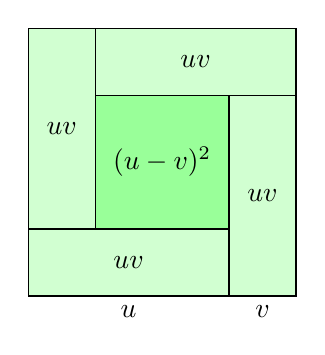
\begin{tikzpicture}[scale=.85]
\foreach \x/\y/\w/\h in {0/0/3/1,3/0/1/3,1/3/3/1,0/1/1/3}{\draw[fill=green!18] (\x,\y) rectangle ++(\w,\h);}
\draw[fill=green!40] (1,1) rectangle (3,3);
\node at (2,2) {$(u-v)^2$};\node at (1.5,.5){$uv$};\node at (3.5,1.5){$uv$};\node at (2.5,3.5){$uv$};\node at (.5,2.5){$uv$};
\node[below] at (1.5,0){$u$};\node[below] at (3.5,0){$v$};
\end{tikzpicture}
\end{center}
图示 $u\ge v$；若 $u<v$，交换两者即可。
\begin{align*}(u+v)^2&=4uv+(u-v)^2\ge4uv,\\
u^2+2uv+v^2&\ge4uv,\\u^2+v^2&\ge2uv,\\a+b&\ge2\sqrt{ab}.\end{align*}
等号当且仅当中心面积为零，即 $u=v$，也就是 $a=b$。零边长情形直接代入亦成立。
\medskip\textbf{补充方法三：二次函数法（定和求积）}
令 $a+b=S$，则 $b=S-a$，因此
\begin{align*}ab&=a(S-a)\\&=-a^2+Sa\\&=-\left(a-\frac S2\right)^2+\frac{S^2}{4}\\&\le\frac{S^2}{4}.\end{align*}
二次函数开口向下，顶点对应 $a=S/2$，此时 $b=S/2$。若无其他约束，积取得最大值。
\begin{center}
\begin{tikzpicture}[every node/.style={draw,rounded corners,align=center,font=\small,inner sep=4pt}]
\node (r) at (0,0) {$(a-b)^2\ge0$};
\node (s) at (0,-1.3) {$a^2+b^2\ge2ab$};
\node (m) at (-2.8,-2.8) {$a+b\ge2\sqrt{ab}$};
\node (q) at (2.8,-2.8) {$a^2+b^2\ge(a+b)^2/2$};
\node (p) at (-2.8,-4.3) {$ab\le(a+b)^2/4$};
\draw[->] (r)--(s) node[midway,right,draw=none]{展开、移项};
\draw[->] (s)--(m) node[midway,left,draw=none]{非负数代换};
\draw[->] (s)--(q) node[midway,right,draw=none]{加项、除以2};
\draw[->] (m)--(p) node[midway,right,draw=none]{平方、除以4};
\end{tikzpicture}
\par 积与和平方的关系另由直接配方推广至任意实数。
\end{center}
\end{proofbox}
